\documentclass[aspectratio=169,10pt]{beamer}
\usetheme{Madrid}
\usepackage[T1]{fontenc}
\usepackage{lmodern}
\usepackage{graphicx,booktabs,amsmath,tikz}
\usetikzlibrary{arrows.meta,positioning,calc}
\definecolor{AvansRed}{HTML}{C5221F}
\definecolor{AvansBlue}{HTML}{233D60}
\definecolor{AvansGrey}{HTML}{5C6670}
\setbeamercolor{structure}{fg=AvansRed}
\setbeamercolor{palette primary}{bg=AvansRed,fg=white}
\setbeamercolor{palette secondary}{bg=AvansRed!80!black,fg=white}
\setbeamercolor{palette tertiary}{bg=AvansBlue,fg=white}
\setbeamercolor{frametitle}{bg=AvansRed,fg=white}
\setbeamercolor{title}{bg=AvansRed,fg=white}
\setbeamercolor{block title}{fg=AvansBlue,bg=AvansBlue!10}
\setbeamercolor{block body}{fg=black,bg=AvansBlue!3}
\setbeamertemplate{navigation symbols}{}
\setbeamertemplate{blocks}[rounded][shadow=false]
\setbeamersize{text margin left=7mm,text margin right=7mm}
\setbeamerfont{block title}{size=\normalsize}
\setbeamerfont{block body}{size=\small}
\setbeamertemplate{footline}{\leavevmode\hbox{%
\begin{beamercolorbox}[wd=.33\paperwidth,ht=2.6ex,dp=1.2ex,leftskip=3mm]{author in head/foot}Avans Aerospace Engineering \& Maintenance\end{beamercolorbox}%
\begin{beamercolorbox}[wd=.45\paperwidth,ht=2.6ex,dp=1.2ex,center]{title in head/foot}Wind tunnel development \textbar\ 8 November 2026\end{beamercolorbox}%
\begin{beamercolorbox}[wd=.22\paperwidth,ht=2.6ex,dp=1.2ex,rightskip=3mm plus1fil]{date in head/foot}\hfill\insertframenumber/\inserttotalframenumber\end{beamercolorbox}}}
\newcommand{\noteunder}[1]{\par\vspace{.35em}{\footnotesize\color{AvansGrey}#1}\par}
\newenvironment{points}{\begin{itemize}\setlength{\itemsep}{.5em}}{\end{itemize}}
\title[Wind tunnel development]{Wind Tunnel Project}
\subtitle{Development progress: architecture, HMI and control comparison}
\author[R. van Eekelen]{Konstantin Nikitin \enspace\textbar\enspace Bas Keultjes\\Dante Bloemendaal \enspace\textbar\enspace Robbe van Eekelen}
\institute{Aerospace Engineering \& Maintenance\\Avans University of Applied Sciences}
\date{8 November 2026}

\begin{document}

\begin{frame}
\vspace{.3cm}
\begin{beamercolorbox}[wd=\linewidth,sep=10pt,center,rounded=true]{title}
{\LARGE Wind Tunnel Project}\par\vspace{.2cm}
{\large Architecture, HMI and control comparison}
\end{beamercolorbox}
\vspace{.45cm}
\begin{center}
Konstantin Nikitin \quad Bas Keultjes\\[.15cm]
Dante Bloemendaal \quad Robbe van Eekelen\\[.4cm]
Aerospace Engineering \& Maintenance\\
Avans University of Applied Sciences\\[.2cm]
8 November 2026\\[.45cm]
{\color{AvansBlue}\bfseries Software demonstrated; physical commissioning pending}
\end{center}
\end{frame}

\begin{frame}{Project objectives and operating envelope}
\begin{columns}[T,onlytextwidth]
\column{.52\textwidth}
\begin{block}{Educational aerodynamic test facility}
\begin{points}
\item Develop the existing open-return tunnel.
\item Control airspeed and record repeatable runs.
\item Measure $C_p(x/c)$ and pressure-derived lift.
\item Compare experiments with XFOIL; explain deviations.
\end{points}
\end{block}
\column{.44\textwidth}
\small\renewcommand{\arraystretch}{1.55}
\begin{tabular}{@{}ll@{}}\toprule
Item & Configured\\\midrule
Airspeed setpoint & $0$--$40\ \mathrm{m/s}$\\
V20 command & $0$--$50\ \mathrm{Hz}$\\
Control cycle & $100\ \mathrm{Hz}$\\
Pitot reporting & approximately $20\ \mathrm{Hz}$\\
Operator interface & Native HMI + local API\\\bottomrule
\end{tabular}
\noteunder{Limits are configured values, not demonstrated tunnel performance. V20 system rating: 5.5 kW.}
\end{columns}
\end{frame}

\begin{frame}{Mechanical integration and airflow quality}
\centering\resizebox{!}{3.6cm}{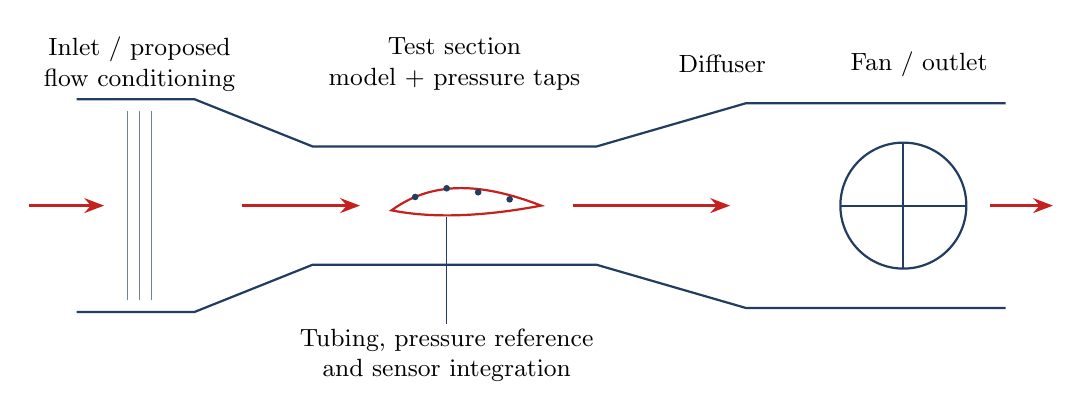
\begin{tikzpicture}[x=1cm,y=1cm,flow/.style={-{Stealth[length=2.5mm]},very thick,AvansRed},lab/.style={font=\small,align=center}]
\draw[thick,AvansBlue] (0,1.35)--(1.5,1.35)--(3,.75)--(6.6,.75)--(8.5,1.3)--(11.8,1.3);
\draw[thick,AvansBlue] (0,-1.35)--(1.5,-1.35)--(3,-.75)--(6.6,-.75)--(8.5,-1.3)--(11.8,-1.3);
\foreach \x in {.65,.8,.95} {\draw[AvansBlue!65] (\x,-1.2)--(\x,1.2);}
\draw[thick,AvansRed] (4,-.06)..controls(4.6,.38)and(5.3,.23)..(5.9,0)..controls(5,-.17)and(4.4,-.14)..cycle;
\foreach \x/\y in {4.3/.11,4.7/.22,5.1/.17,5.5/.08} {\fill[AvansBlue] (\x,\y) circle(1.2pt);}
\draw[AvansBlue,thick] (10.5,0) circle(.8);
\draw[AvansBlue,thick] (10.5,-.8)--(10.5,.8) (9.7,0)--(11.3,0);
\draw[flow] (-.6,0)--(.35,0); \draw[flow] (2.1,0)--(3.6,0); \draw[flow] (6.3,0)--(8.3,0); \draw[flow] (11.6,0)--(12.4,0);
\node[lab] at (.8,1.8) {Inlet / proposed\\flow conditioning};
\node[lab] at (4.8,1.8) {Test section\\model + pressure taps};
\node[lab] at (8.2,1.8) {Diffuser};
\node[lab] at (10.7,1.8) {Fan / outlet};
\draw[AvansBlue] (4.7,-.15)--(4.7,-1.5);
\node[lab] at (4.7,-1.9) {Tubing, pressure reference\\and sensor integration};
\end{tikzpicture}
}
\noteunder{Functional concept only: not an as-built drawing and not to scale.}
\vspace{.25em}
\begin{columns}[T,onlytextwidth]
\column{.48\textwidth}\begin{block}{Existing structure}
\small Open-return tunnel; integrate the airfoil, pressure taps, tubing and a stable reference pressure.
\end{block}
\column{.48\textwidth}\begin{block}{Inspection priorities}
\small Recheck leaks, door closure and flow conditioning identified in the workplan; then measure flow uniformity.
\end{block}
\end{columns}
\end{frame}

\begin{frame}{Electrical cabinet and embedded architecture}
\begin{columns}[c,onlytextwidth]
\column{.64\textwidth}
\centering\resizebox{!}{4.8cm}{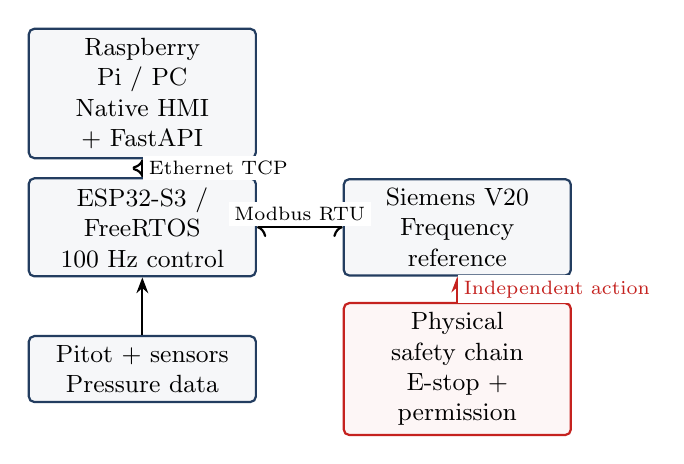
\begin{tikzpicture}[x=1cm,y=1cm,
unit/.style={draw=AvansBlue,thick,rounded corners=2pt,fill=AvansBlue!4,align=center,font=\small,text width=2.65cm,minimum height=.8cm},
flow/.style={-{Stealth[length=2mm]},thick},lab/.style={font=\scriptsize,fill=white,inner sep=2pt}]
\node[unit] (hmi) at (0,0) {Raspberry Pi / PC\\Native HMI + FastAPI};
\node[unit] (esp) at (0,-1.7) {ESP32-S3 / FreeRTOS\\100 Hz control};
\node[unit] (vfd) at (4,-1.7) {Siemens V20\\Frequency reference};
\node[unit] (sensor) at (0,-3.5) {Pitot + sensors\\Pressure data};
\node[unit,draw=AvansRed,fill=AvansRed!4] (safety) at (4,-3.5) {Physical safety chain\\E-stop + permission};
\draw[flow,<->] (hmi)--node[lab,right]{Ethernet TCP}(esp);
\draw[flow,<->] (esp)--node[lab,above]{Modbus RTU}(vfd);
\draw[flow] (sensor)--(esp);
\draw[flow,AvansRed] (safety)--node[lab,right]{Independent action}(vfd);
\end{tikzpicture}
}
\noteunder{100 Hz control; sensor/control phases separated by 5 ms.\newline Physical START/STOP/RESET and safety feedback enter the ESP32.}
\column{.32\textwidth}
\centering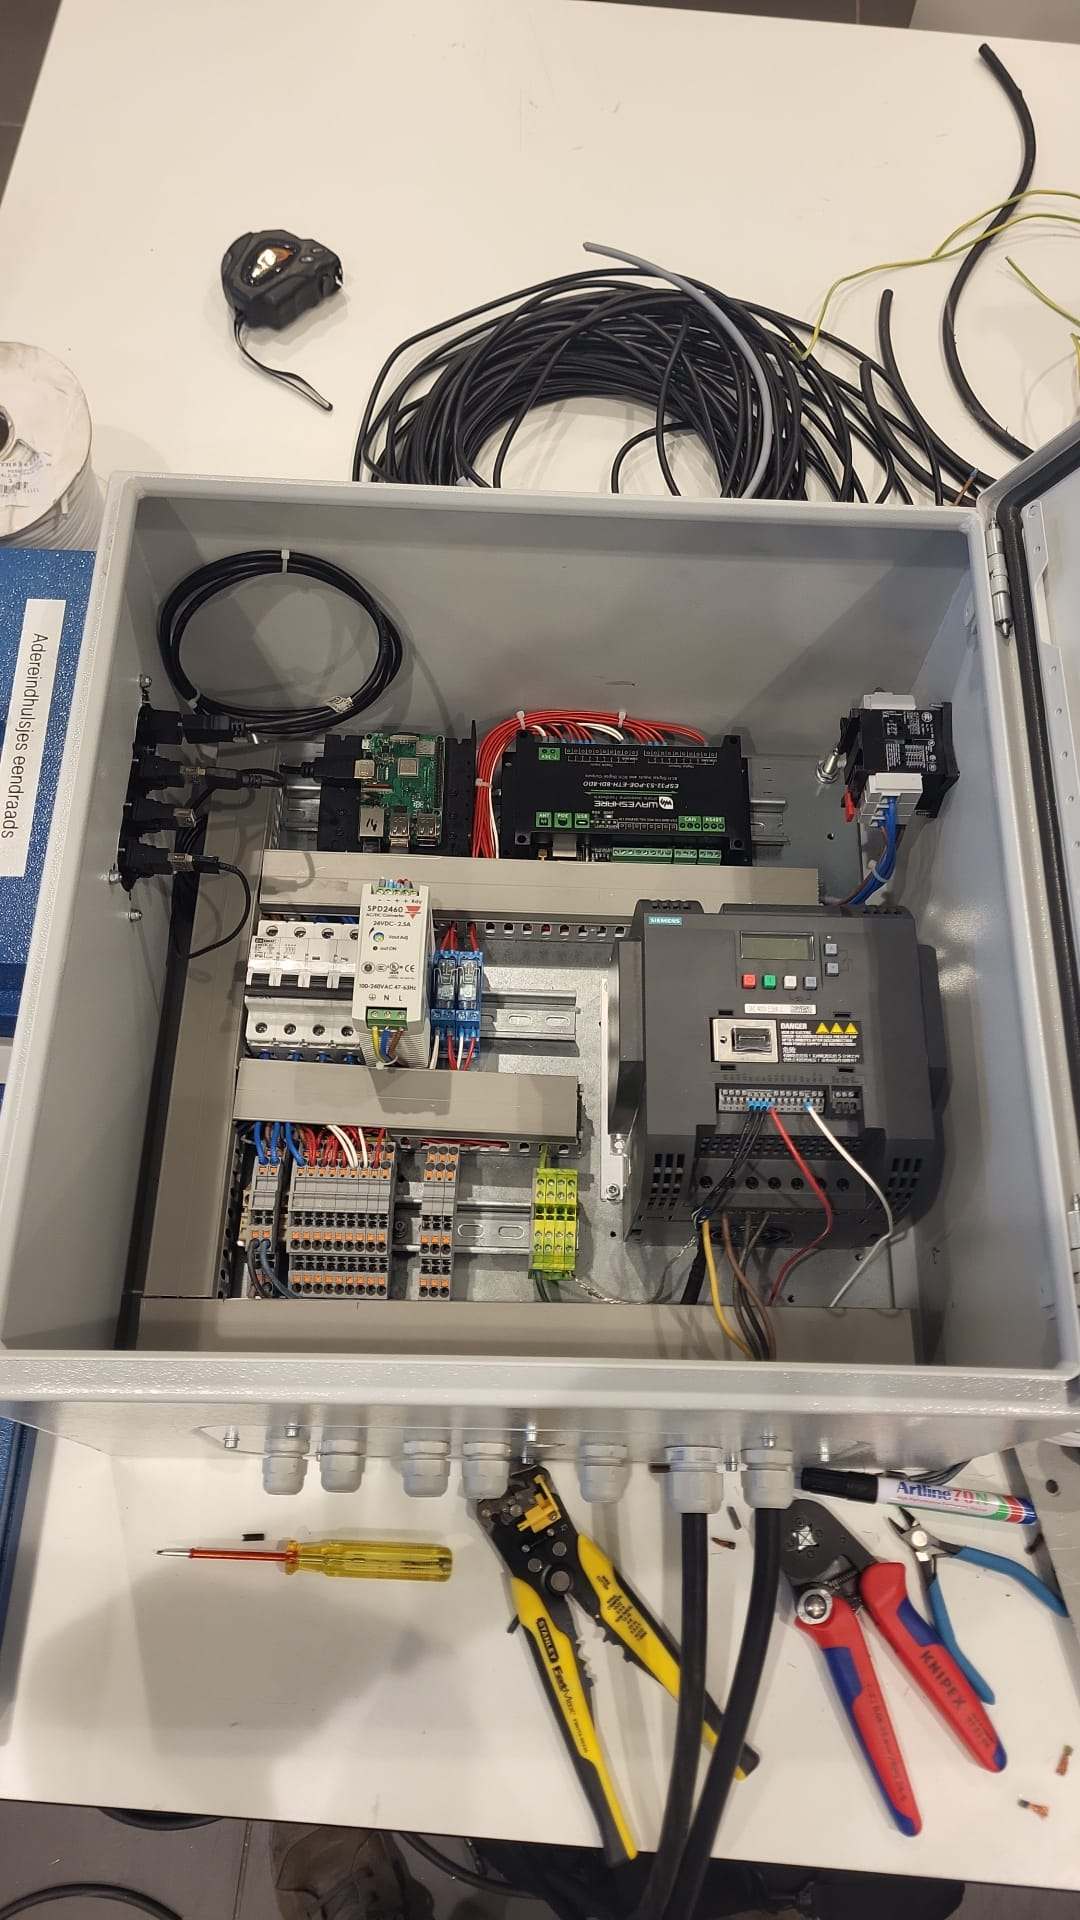
\includegraphics[width=\linewidth,trim=0 390 0 400,clip]{assets/new_cabinet.jpg}
\noteunder{New cabinet -- supplied project photo. Assembly progress; commissioning pending.}
\end{columns}
\end{frame}

\begin{frame}{Current native HMI}
\begin{columns}[T,onlytextwidth]
\column{.72\textwidth}
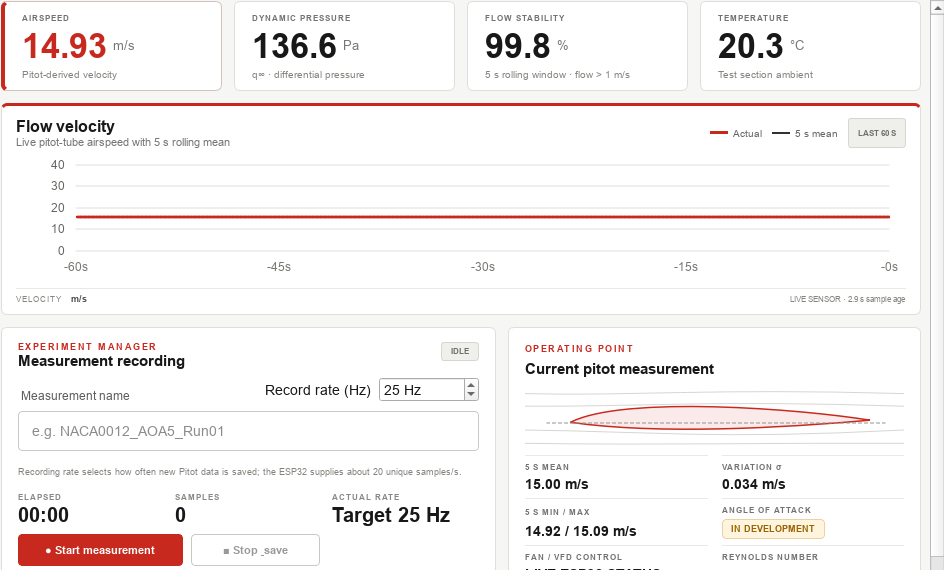
\includegraphics[width=\linewidth,height=4.65cm,keepaspectratio]{assets/hmi_dashboard.png}
\noteunder{Dashboard: airspeed, pressure, stability, recording and operating point.}
\column{.24\textwidth}
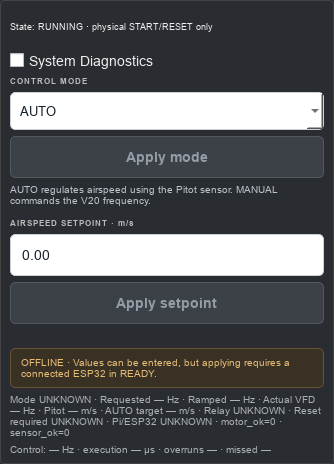
\includegraphics[width=\linewidth,height=4.65cm,keepaspectratio]{assets/hmi_control.png}
\noteunder{AUTO / MANUAL.\newline Physical START/RESET required.}
\end{columns}
\noteunder{Actual widgets with \textbf{simulated telemetry}; no hardware connection.}
\end{frame}

\begin{frame}{V20 startup, OFF1/OFF2 and safety}
\centering\resizebox{.98\textwidth}{!}{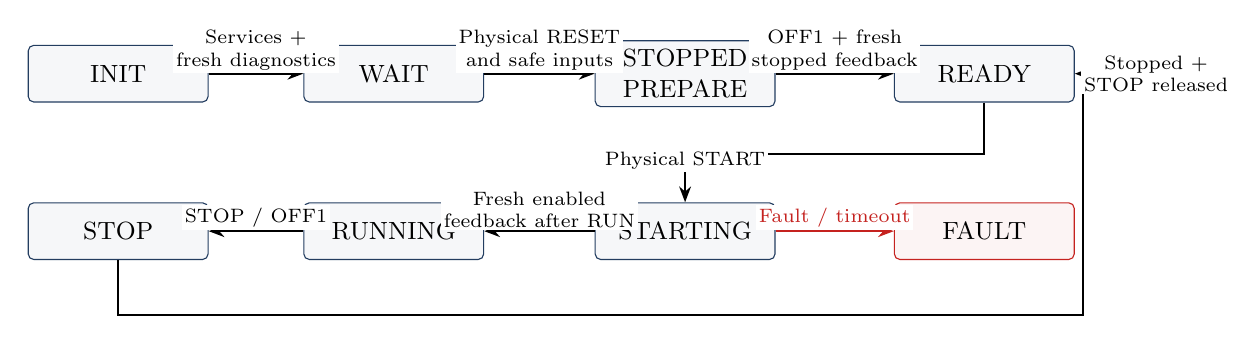
\begin{tikzpicture}[x=1cm,y=1cm,
state/.style={draw=AvansBlue,fill=AvansBlue!4,rounded corners=2pt,align=center,font=\small,minimum height=.72cm,text width=2.05cm},
flow/.style={-{Stealth[length=2mm]},thick},lab/.style={font=\scriptsize,align=center,fill=white,inner sep=1pt}]
\node[state] (init) at (0,0) {INIT};
\node[state] (wait) at (3.5,0) {WAIT};
\node[state] (prep) at (7.2,0) {STOPPED\\PREPARE};
\node[state] (ready) at (11,0) {READY};
\node[state] (stop) at (0,-2) {STOP};
\node[state] (run) at (3.5,-2) {RUNNING};
\node[state] (start) at (7.2,-2) {STARTING};
\node[state,draw=AvansRed,fill=AvansRed!5] (fault) at (11,-2) {FAULT};
\draw[flow] (init)--node[lab,above]{Services +\\fresh diagnostics}(wait);
\draw[flow] (wait)--node[lab,above]{Physical RESET\\and safe inputs}(prep);
\draw[flow] (prep)--node[lab,above]{OFF1 + fresh\\stopped feedback}(ready);
\draw[flow] (ready.south)--++(0,-.65)-|node[lab,pos=.7,above]{Physical START}(start.north);
\draw[flow] (start)--node[lab,above]{Fresh enabled\\feedback after RUN}(run);
\draw[flow] (run)--node[lab,above]{STOP / OFF1}(stop);
\draw[flow] (stop.south)--++(0,-.7)--++(12.25,0)|-node[lab,pos=.65,right]{Stopped +\\STOP released}(ready.east);
\draw[flow,AvansRed] (start)--node[lab,above]{Fault / timeout}(fault);
\end{tikzpicture}
}
\vspace{.5em}
\begin{columns}[T,onlytextwidth]
\column{.48\textwidth}\small
\textbf{Stopped preparation}\begin{itemize}
\item OFF1: \texttt{0x047E}; normal ramp stop.
\item Intended DO1/In1 path releases OFF2 after RESET and acknowledged OFF1.
\end{itemize}
\column{.48\textwidth}\small
\textbf{Feedback-confirmed start}\begin{itemize}
\item Physical START: \texttt{0x047F}, initially zero setpoint.
\item RUNNING requires fresh operation-enabled feedback; 5 s start timeout.
\end{itemize}
\end{columns}
\noteunder{OFF3 is kept inactive for normal operation. Applicable faults inhibit RUN; physical safety remains independent. RESET returns to stopped recovery, never automatic restart.}
\end{frame}

\begin{frame}{Two control approaches, one V20 frequency interface}
\centering\resizebox{!}{3.8cm}{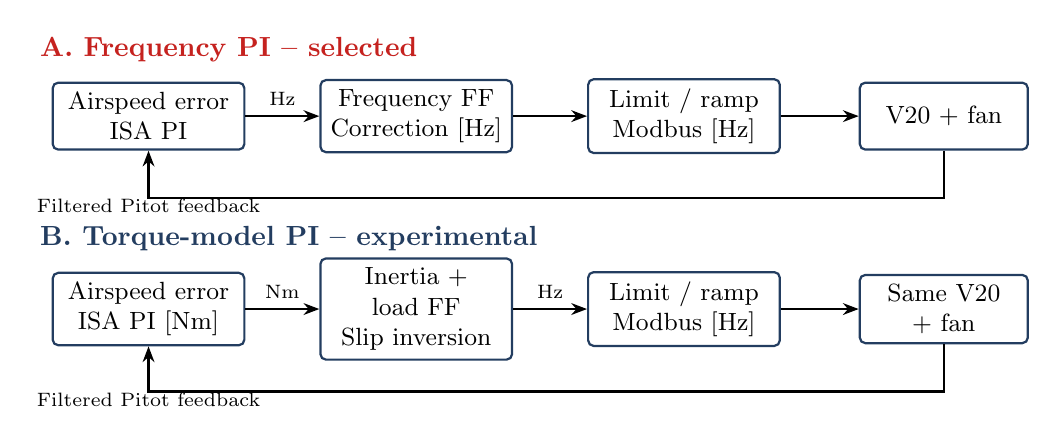
\begin{tikzpicture}[x=1cm,y=1cm,
unit/.style={draw=AvansBlue,thick,rounded corners=2pt,align=center,font=\small,minimum height=.85cm},
flow/.style={-{Stealth[length=2mm]},thick},lab/.style={font=\scriptsize,align=center}]
\node[anchor=west,text=AvansRed,font=\normalsize\bfseries] at (-.8,.85) {A. Frequency PI -- selected};
\node[unit,text width=2.2cm] (a1) at (.7,0) {Airspeed error\\ISA PI};
\node[unit,text width=2.2cm] (a2) at (4.1,0) {Frequency FF\\Correction [Hz]};
\node[unit,text width=2.2cm] (a3) at (7.5,0) {Limit / ramp\\Modbus [Hz]};
\node[unit,text width=1.9cm] (a4) at (10.8,0) {V20 + fan};
\draw[flow] (a1)--node[lab,above]{Hz}(a2); \draw[flow] (a2)--(a3); \draw[flow] (a3)--(a4);
\draw[flow] (a4.south)--++(0,-.6)-|node[lab,pos=.6,below]{Filtered Pitot feedback}(a1.south);
\node[anchor=west,text=AvansBlue,font=\normalsize\bfseries] at (-.8,-1.55) {B. Torque-model PI -- experimental};
\node[unit,text width=2.2cm] (b1) at (.7,-2.45) {Airspeed error\\ISA PI [Nm]};
\node[unit,text width=2.2cm] (b2) at (4.1,-2.45) {Inertia + load FF\\Slip inversion};
\node[unit,text width=2.2cm] (b3) at (7.5,-2.45) {Limit / ramp\\Modbus [Hz]};
\node[unit,text width=1.9cm] (b4) at (10.8,-2.45) {Same V20 + fan};
\draw[flow] (b1)--node[lab,above]{Nm}(b2); \draw[flow] (b2)--node[lab,above]{Hz}(b3); \draw[flow] (b3)--(b4);
\draw[flow] (b4.south)--++(0,-.6)-|node[lab,pos=.6,below]{Filtered Pitot feedback}(b1.south);
\end{tikzpicture}
}
\vspace{.4em}
\small
\begin{columns}[T,onlytextwidth]
\column{.48\textwidth}\textbf{Frequency PI}: fewer uncertain physical parameters; identified Hz-to-airspeed model and measured fan characteristic required.
\column{.48\textwidth}\textbf{Torque model}: inertia/load feedforward and slip inversion; more parameter dependence. Physical torque-model actuation remains disabled.
\end{columns}
\noteunder{Both use digital ISA control with Tustin integration. The present comparison uses \textbf{PI}, not active derivative action. The V20 receives \textbf{Hz}, not torque commands.}
\end{frame}

\begin{frame}{Simulated airspeed tracking: shared physical plant}
\centering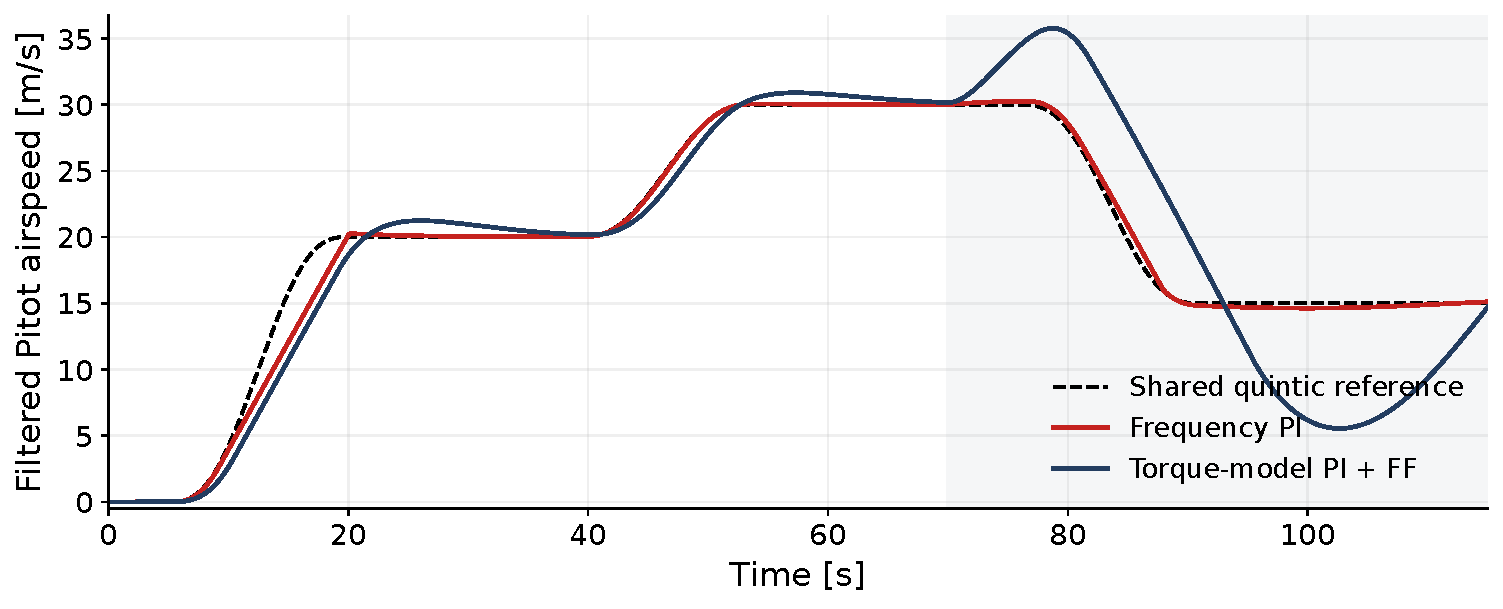
\includegraphics[width=.98\textwidth,height=4.9cm,keepaspectratio]{plots/airspeed_response.pdf}
\vspace{-.15em}
\begin{columns}[T,onlytextwidth]\small
\column{.48\textwidth}
Same initial state; $0\!\to\!20\!\to\!30\!\to\!15$ m/s profiles; 100 Hz; 1 Hz Pitot pressure filter.
\column{.48\textwidth}
Same $J=0.3712$ kg\,m$^2$, nonlinear motor/fan plant, $0$--$50$ Hz limit and assumed $2$ Hz/s drive ramp.
\end{columns}
\noteunder{Supplied Python calculation, unchanged defaults. Shading marks a 1 m/s, 0.02 Hz output disturbance from 70 s. Motor/slip/ramp values are unvalidated assumptions.}
\end{frame}

\begin{frame}{Control demand, error and interpretation}
\begin{columns}[T,onlytextwidth]
\column{.49\textwidth}\centering
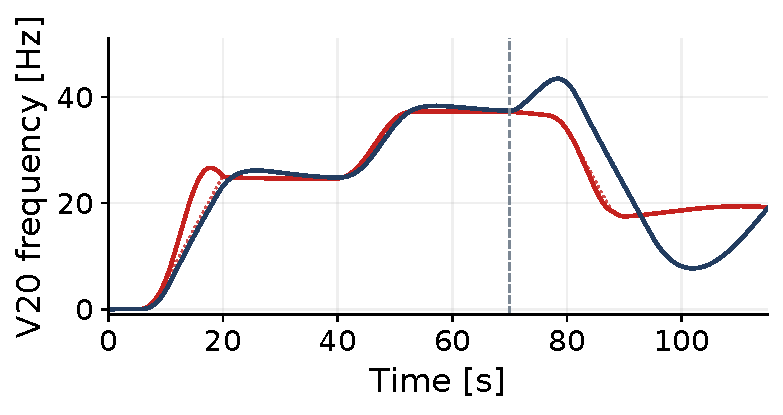
\includegraphics[width=\linewidth,height=3.05cm,keepaspectratio]{plots/frequency_output.pdf}
\column{.49\textwidth}\centering
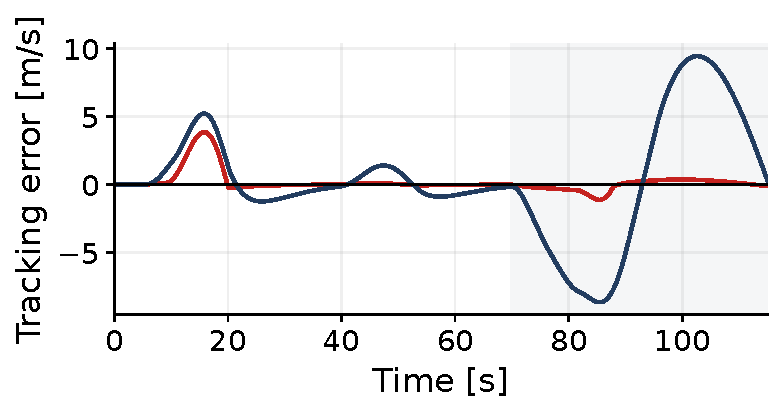
\includegraphics[width=\linewidth,height=3.05cm,keepaspectratio]{plots/disturbance_error.pdf}
\end{columns}
\vspace{-.2em}
\small\centering\renewcommand{\arraystretch}{1.15}
\begin{tabular}{@{}lrrrr@{}}\toprule
 & Rise [s] & Settle [s] & MAE$_{25-38\,s}$ & MAE$_{99-114\,s}$\\\midrule
Frequency PI & 9.88 & 14.66 & 0.04 & 0.22 \\
Torque model & 9.97 & 30.59 & 0.79 & 7.15 \\
\bottomrule\end{tabular}

\noteunder{Red: frequency PI; blue: torque-model PI. Dotted: actual Hz. MAE: m/s. Rise: 10--90\%; settle: $\pm2\%$ from $t=5$~s.}
\noteunder{Frequency PI tracks better with these provisional tunings. Feedforward differs; the late window includes a down-transition and disturbance. Hardware validation remains pending.}
\end{frame}

\begin{frame}{Aerodynamic acquisition and $C_p/C_l$ analysis}
\begin{columns}[T,onlytextwidth]
\column{.40\textwidth}
\begin{points}
\item Pair pressure taps with fresh reference pressure and airspeed.
\item Validate channels and integrate pressure over known geometry.
\item Compare runs by angle of attack and data source.
\end{points}
\vspace{.4em}
$\displaystyle C_p=\frac{p-p_\infty}{\tfrac12\rho V_\infty^2}$
\column{.57\textwidth}
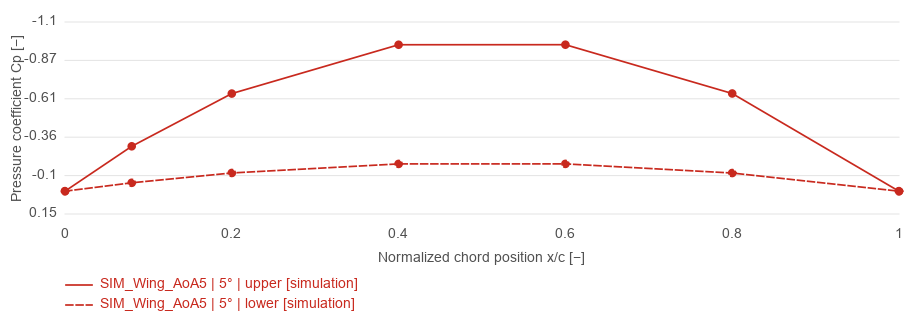
\includegraphics[width=\linewidth]{assets/hmi_cp_plot.png}
\noteunder{Actual analytics widget: synthetic diamond section, $\alpha=5^\circ$, 14 simulated taps. Not an experimental airfoil result.}
\begin{block}{Implemented quality gates}
\small Pressure-derived sectional lift/moment only when geometry and data are sufficient. Total drag is not available from pressure alone.
\end{block}
\end{columns}
\noteunder{Physical pressure acquisition still needs a configured, validated adapter; real sensor channels and tubing require calibration.}
\end{frame}

\begin{frame}{Software validation and project progress}
\begin{columns}[T,onlytextwidth]
\column{.48\textwidth}
\small\renewcommand{\arraystretch}{1.6}
\begin{tabular}{@{}lr@{}}\toprule
Validation & Passing result\\\midrule
Host regression executables & 23 / 23\\
Firmware build variants & 3 / 3\\
HMI unit/integration tests & 104\\
I/O configuration checks & 7\\
Migration checks & 7\\\bottomrule
\end{tabular}
\noteunder{Recorded results from software update \texttt{b130348}. No physical actuation.}
\column{.48\textwidth}
\begin{block}{Demonstrated in software}
\small Fresh-start and reset handling; fault lockout; bounded STOP attempts; delayed-reply rejection; stateful drive simulation; HMI acquisition/analysis.
\end{block}
\begin{block}{Installation checks still open}
\small DO1/OFF2 wiring and BICO settings; independent safety circuit; V20 watchdog and restart behavior; real sensors, airflow and dynamics.
\end{block}
\end{columns}
\end{frame}

\begin{frame}{Next steps and conclusions}
\begin{enumerate}\setlength{\itemsep}{.7em}
\item Verify cabinet wiring, independent safety and V20 OFF2/watchdog behavior with the motor isolated.
\item Identify actual frequency dynamics and validate the stored fan calibration.
\item Commission controlled starts/stops, sensor channels and airflow quality.
\item Acquire repeatable $C_p$ data and compare with XFOIL and uncertainty bounds.
\end{enumerate}
\vfill
\begin{block}{Current maturity}
\centering Software and HMI extensively tested; new cabinet assembled.\\
Physical commissioning and experimental aerodynamic validation remain pending.
\end{block}
\end{frame}
\end{document}
